% fig_ar_timeline.tex
% TR-36: AR event timeline — fault inception to reclose (successful and failed)
%
% Two swim-lanes: (a) transient fault (successful AR), (b) permanent fault
%
% Scale: 1 cm = 50 ms
% Key times (k_ibr = 0.15, T_dead = 205 ms):
%   0 ms   : fault inception
%  20 ms   : first trip (Z1 / 87L)
%  70 ms   : CB fully open (first trip + 50 ms opening)
%  70 ms   : T_mem start countdown (100 ms window)
% 170 ms   : T_mem expires
% 275 ms   : reclose (70 + 205 ms dead time)
% 295 ms   : CB fully closed
% 295 ms   : (a) transient: line healthy → no second trip → service restored
% 295 ms   : (b) permanent: fault re-applies → second trip by 87L at 315 ms
% 315 ms   : 87L second trip (memory expired, Z1/POTT unavailable)
% 345 ms   : lock-out

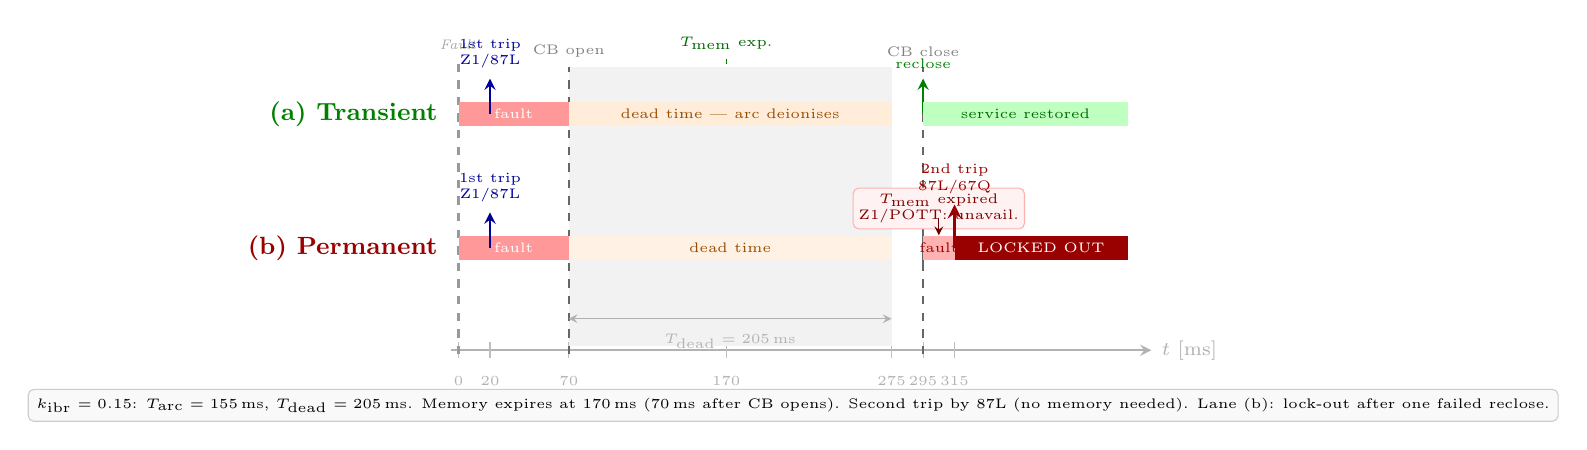
\begin{tikzpicture}[every node/.style={font=\scriptsize}]

%% ── Scale: 1cm = 50ms ────────────────────────────────────────────────────────
% Hardcoded x-positions (cm):
% xF=0, xTrip=0.40, xOpen=1.40, xMem=3.40, xDead=5.50, xClose=5.90
% xSecTrip=6.30, xLock=7.30
% xEnd=8.50

%% ── Lane y-positions ─────────────────────────────────────────────────────────
% yTrans=2.5 (transient), yPerm=0.8 (permanent), yAx=-0.5

%% ── Time axis ────────────────────────────────────────────────────────────────
\draw[->, >=stealth, gray!60, thick]
  (-0.10, -0.5) -- (8.80, -0.5) node[right, gray!60] {$t$ [ms]};

\foreach \xpos/\lab in {0/0, 0.40/20, 1.40/70, 3.40/170, 5.50/275, 5.90/295, 6.30/315}{
  \draw[gray!50, thin] (\xpos, -0.60) -- (\xpos, -0.40);
  \node[gray!60, below=3pt, font=\tiny] at (\xpos, -0.60) {\lab};
}

%% ── Fault inception ──────────────────────────────────────────────────────────
\draw[gray!80, thick, dashed] (0, -0.55) -- (0, 3.20);
\node[gray!70, above, font=\tiny] at (0, 3.20) {\textit{Fault}};

%% ── Memory window ────────────────────────────────────────────────────────────
\fill[green!8] (1.40, -0.45) rectangle (3.40, 3.10);
\draw[green!50!black, dashed] (3.40, -0.45) -- (3.40, 3.20);
\node[green!40!black, font=\tiny, above] at (3.40, 3.20) {$T_\mathrm{mem}$ exp.};

%% ── Dead time shading ────────────────────────────────────────────────────────
\fill[gray!10] (1.40, -0.45) rectangle (5.50, 3.10);

%% ── CB open / close markers ──────────────────────────────────────────────────
\draw[black!60, thick, dashed] (1.40, -0.55) -- (1.40, 3.10);
\node[black!50, font=\tiny, above] at (1.40, 3.10) {CB open};
\draw[black!60, thick, dashed] (5.90, -0.55) -- (5.90, 3.10);
\node[black!50, font=\tiny, above] at (5.90, 3.10) {CB close};

%% ── LANE LABELS ──────────────────────────────────────────────────────────────
\node[green!50!black, font=\small\bfseries, left=4pt] at (0, 2.5)
  {(a) Transient};
\node[red!60!black,   font=\small\bfseries, left=4pt] at (0, 0.8)
  {(b) Permanent};

%% ═══ LANE A: TRANSIENT FAULT ═════════════════════════════════════════════════

%% Fault current bar
\fill[red!40] (0, 2.35) rectangle (1.40, 2.65);
\node[white, font=\tiny] at (0.70, 2.50) {fault};

%% First trip marker
\draw[blue!60!black, ->, >=stealth, thick]
  (0.40, 2.50) -- (0.40, 2.95)
  node[above, blue!60!black, font=\tiny, align=center] {1st trip\\Z1/87L};

%% Dead time (arc quenches)
\fill[orange!15] (1.40, 2.35) rectangle (5.50, 2.65);
\node[orange!60!black, font=\tiny] at (3.45, 2.50) {dead time — arc deionises};

%% Reclose + restoration
\draw[green!50!black, ->, >=stealth, thick]
  (5.90, 2.50) -- (5.90, 2.95)
  node[above, green!50!black, font=\tiny] {reclose};
\fill[green!25] (5.90, 2.35) rectangle (8.50, 2.65);
\node[green!40!black, font=\tiny] at (7.20, 2.50) {service restored};

%% ═══ LANE B: PERMANENT FAULT ════════════════════════════════════════════════

%% First fault current bar
\fill[red!40] (0, 0.65) rectangle (1.40, 0.95);
\node[white, font=\tiny] at (0.70, 0.80) {fault};

%% First trip
\draw[blue!60!black, ->, >=stealth, thick]
  (0.40, 0.80) -- (0.40, 1.25)
  node[above, blue!60!black, font=\tiny, align=center] {1st trip\\Z1/87L};

%% Dead time
\fill[orange!10] (1.40, 0.65) rectangle (5.50, 0.95);
\node[orange!60!black, font=\tiny] at (3.45, 0.80) {dead time};

%% Reclose onto permanent fault
\draw[black!60, thick] (5.90, 0.55) -- (5.90, 1.05);
\fill[red!30] (5.90, 0.65) rectangle (6.30, 0.95);
\node[red!60!black, font=\tiny] at (6.10, 0.80) {fault};

%% Memory expired annotation
\node[red!50!black, font=\tiny, align=center, draw=red!30, fill=red!5,
      rounded corners=2pt, inner sep=2pt]
  at (6.10, 1.30) {$T_\mathrm{mem}$ expired\\Z1/POTT: unavail.};
\draw[->, >=stealth, red!40!black, thin] (6.10, 1.18) -- (6.10, 0.96);

%% Second trip by 87L
\draw[red!60!black, ->, >=stealth, very thick]
  (6.30, 0.80) -- (6.30, 1.35)
  node[above, red!60!black, font=\tiny, align=center] {2nd trip\\87L/67Q};

%% Lock-out
\fill[red!60!black] (6.30, 0.65) rectangle (8.50, 0.95);
\node[white, font=\tiny] at (7.40, 0.80) {LOCKED OUT};

%% ── Dead time annotation ─────────────────────────────────────────────────────
\draw[<->, >=stealth, gray!60]
  (1.40, -0.10) -- (5.50, -0.10)
  node[midway, below=2pt, font=\tiny, gray!60] {$T_\mathrm{dead}=205$\,ms};

%% ── Caption ──────────────────────────────────────────────────────────────────
\node[draw=gray!40, fill=gray!5, rounded corners=2pt,
      font=\tiny, inner sep=3pt, align=center]
  at (4.25, -1.2)
  {$k_\mathrm{ibr}=0.15$: $T_\mathrm{arc}=155$\,ms, $T_\mathrm{dead}=205$\,ms.
   Memory expires at 170\,ms (70\,ms after CB opens).
   Second trip by 87L (no memory needed). Lane~(b): lock-out after one failed reclose.};

\end{tikzpicture}
